%%%%%%%%%%%%%%%%%%%%%%%%%%%%%%%%%%%%%%%%%%  不使用 authblk 包制作标题  %%%%%%%%%%%%%%%%%%%%%%%%%%%%%%%%%%%%%%%%%%%%%%
%-------------------------------PPT Title-------------------------------------
\title{拟入表资产介绍}
%\substitle{}
%-----------------------------------------------------------------------------

%----------------------------Author & Date------------------------------------
%\author[\textrm{Jun\_Jiang}]{姜\;\;骏\inst{}} %[]{} (optional, use only with lots of authors)
%% - Give the names in the same order as the appear in the paper.
%% - Use the \inst{?} command only if the authors have different
%%   affiliation.
\institute[BCC]{\inst{}%
%\institute[Gain~Strong]{\inst{}%
\vskip 3pt 北京市计算中心}
%云平台事业部~材料计算团队}
%\vskip -20pt {\large 格致斯创~科技}}
\date[\today] % (optional, should be abbreviation of conference name)
{	%{\fontsize{6.2pt}{4.2pt}\selectfont{\textcolor{blue}{E-mail:~}\url{jiangjun@bcc.ac.cn}}}
\vskip 15 pt {\fontsize{8.2pt}{6.2pt}\selectfont{%清华大学\;\;物理系% 报告地点
	\vskip 5 pt \textrm{2024.12}}}
}

%% - Either use conference name or its abbreviation
%% - Not really information to the audience, more for people (including
%%   yourself) who are reading the slides onlin%%   yourself) who are reading the slides onlin%%   yourself) who are reading the slides onlineee
%%%%%%%%%%%%%%%%%%%%%%%%%%%%%%%%%%%%%%%%%%%%%%%%%%%%%%%%%%%%%%%%%%%%%%%%%%%%%%%%%%%%%%%%%%%%%%%%%%%%%%%%%%%%%%%%%%%%%

\subject{}
% This is only inserted into the PDF information catalog. Can be left
% out.
%\maketitle
\frame
{
%	\frametitle{\fontsize{9.5pt}{5.2pt}\selectfont{\textcolor{orange}{“大数据中心调研座谈会”}}}
\titlepage
}
%-----------------------------------------------------------------------------

%------------------------------------------------------------------------------列出全文 outline ---------------------------------------------------------------------------------
\section*{}
\frame[allowframebreaks]
{
  \frametitle{Outline}
%  \frametitle{\textcolor{mycolor}{\secname}}
  \tableofcontents%[current,currentsection,currentsubsection]
}
%在每个section之前列出全部Outline
%类似的在每个subsection之前列出全部Outline是\AtBeginSubsection[]
%\AtBeginSection[]
%{
%  \frame<handout:0>%[allowframebreaks]
%  {
%    \frametitle{Outline}
%%全部Outline中,本部分加亮
%    \tableofcontents[current,currentsection]
%  }
%}

%-----------------------------------------------PPT main Body------------------------------------------------------------------------------------
\small
\section{数据简介}
\frame
{\frametitle{数据资产名称和内容简述}
\begin{itemize}
	\item \textcolor{blue}{数据资产名称:~}北京-稀土与碱土金属化合物、半导体材料电子结构数据
	\item \textcolor{blue}{内容简述}\\
		通过第一原理和分子动力学软件建模并产生的电子结构数据和光学、磁学性质数据,包括:\\
		(1)稀土化合物\textrm{\ch{EuB6}}、\textrm{\ch{EuTe}}的能带和可见-紫外光谱\\
		(2)碱土化合物\textrm{\ch{CaB6}}和金属\textrm{\ch{Pt}}的电子结构数据\\
		(3)过渡金属氧化物\textrm{\ch{NiO}}、\textrm{\ch{CuO}}的基态能量和磁性数据\\
		(4)金属氧化物\textrm{\ch{Al2O3}}的基态能量数据\\
		以及半导体材料\textrm{\ch{Si}}、\textrm{\ch{SiO2}}、\textrm{\ch{GaN}}等的电子结构(能带数据)\\
		高温镍基单晶\textrm{\ch{Ni3Al}}及其铝合金材料的基态能量数据\\
		金属铝、金属铁的分子动力学模拟基础数据
	\item \textcolor{blue}{数据更新频率:~}每年
	\item \textcolor{blue}{数据总量:~}数据规模:~4161个/数据大小:~2\textrm{GB}
\end{itemize}
}

\frame
{\frametitle{数据业务种类}
\begin{itemize}
   		\setlength{\itemsep}{15pt}
		\item \textcolor{blue}{数据分类:~}科研类数据
		\item \textcolor{blue}{数据二次加工情况:~}原始数据
		\item \textcolor{blue}{数据类型:~}少量结构化数据+大量非结构化数据
\end{itemize}
}

\section{数据资产的产生过程}
\frame[allowframebreaks]
{\frametitle{数据资产的产生过程}
\begin{itemize}
	\item 支撑项目(1):~{\fontsize{8.2pt}{6.2pt}\selectfont{国家重点研发计划项目~(\textcolor{red}{已结题})}}
		\vskip 2pt
		“高通量并发式材料计算算法和软件”
		\vskip 2pt
		{\fontsize{8.2pt}{4.2pt}\selectfont{项目编号:~\textrm{2017YFB0701500}}}~ {\fontsize{8.2pt}{6.2pt}\selectfont{执行时间:~\textrm{2017.07-2021.06}}}
	\item 支撑项目(2):~{\fontsize{8.2pt}{6.2pt}\selectfont{内部课题:~``材料计算一体机''(\textcolor{red}{已结题})}}
		\vskip 2pt
		{\fontsize{8.2pt}{4.2pt}\selectfont{项目编号:~单位内部自立项目,无项目编号}}~ {\fontsize{8.2pt}{6.2pt}\selectfont{执行时间:~\textrm{2022.04-2023.03}}}
	\item 数据来源及收集方式:\\
		(1)承担科研项目与任务中要求完成的计算、测试产生的材料计算数据\\
	(2)与北京科技大学、北京航空航天大学、北京师范大学相关课题组老师交流、合作中产生的材料模型实施计算产生的数据
\item 人力成本\\
	 2017-2023年期间,计算材料数据主要由姜骏完成\\
	 2023-2024年,计算材料数据主要由姜骏、高朋林、李鸿飞共同完成
 \item  设备与资源投入:\\
	 \textrm{Lenovo-Think~System SR950-4U}机架式服务器\\
	 8颗\textrm{Intel C624芯片组:~Xeon Platinum 8153至强/内存/主频~2.0G,16核}\\
	 内存\textrm{TruDDR 2666MHz}32根\\
	 硬盘\textrm{240G支持24个磁盘阵列}
 \item  设计的计算平台:\\
	 自研``混合架构材料计算平台''+开源的材料计算与数据处理软件\textrm{Materials~Projects/ASE}
 \item 算法:~通用的微观材料模拟第一原理与分子动力学算法\\
 \item 软件:~开源材料第一原理与分子动力学模拟软件:~\textrm{ABINIT/Elk/Quantum-Espresso/LAMMPS}和跨系统工具开发软件\textrm{Python3.12}等\\
 \item 知识产权:~获得发明专利``晶体对称性及能带路径确定方法及装置''(专利号:~\textrm{ZL202110626051.5})与软件著作权``材料计算自动流程与数据管理软件''(登记号:~\textrm{2023SR0536269})
\begin{figure}[h!]
\centering
\vskip -5pt
\includegraphics[height=1.3in,width=1.0in]{/home/jun-jiang/BCC/年度工作/职称/05-专利.png}
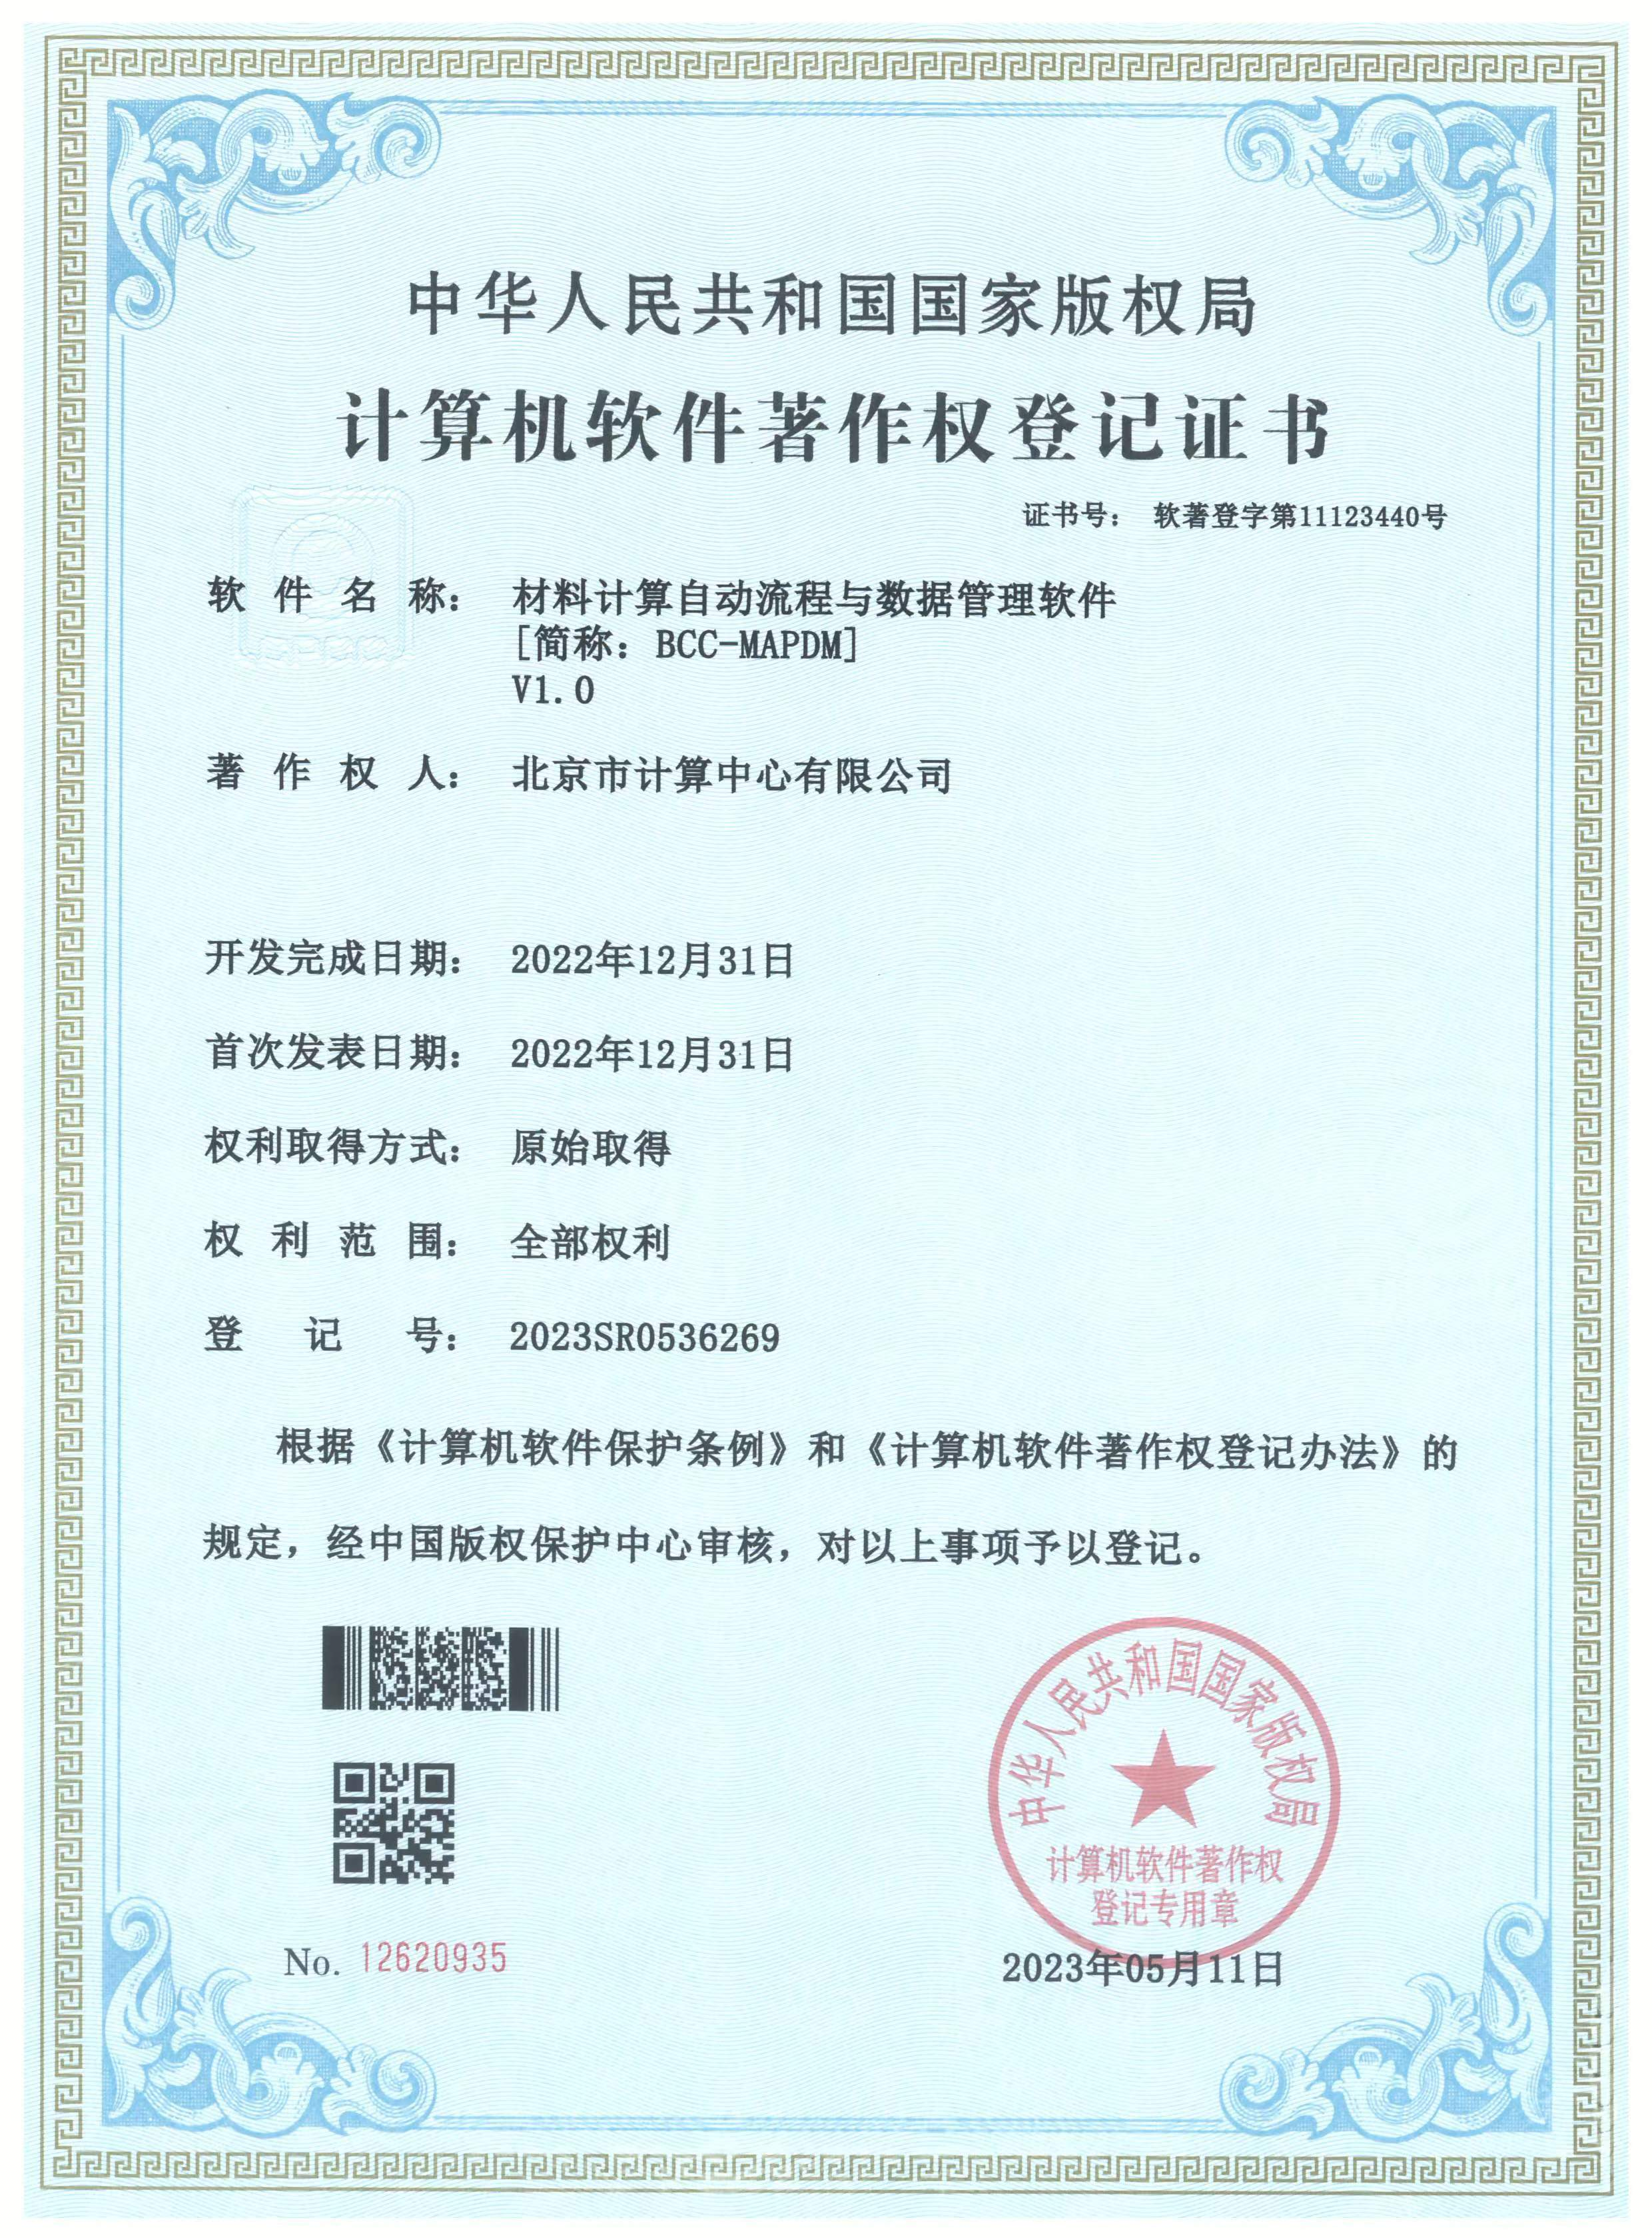
\includegraphics[height=1.3in,width=1.0in]{/home/jun-jiang/BCC/1-著作权/BCC-MAPDM.jpeg}
\label{Fig:Patent}
%\caption{\fontsize{5.2pt}{6.2pt}\selectfont{$\vec k\cdot\vec p$方法保证计算精度,并计算效率提升}}%
\end{figure}
 \item 数据处理的技术手段:\\
	 材料数据主要以文本数据为主,有少量图片及动态/动画数据,一般通过开源软件自带工具和开源可视化工具\textrm{VMD}处理,实现材料物理数据的可视化与动画
 \item 数据处理的方法:~无特殊处理
\end{itemize}
}

\section{数据交易情况}
\frame
{
	\frametitle{数据交易情况}
	数据资产已经提交``北京大数据交易中心''备案,完成``数据知识产权登记''
	\begin{itemize}
		\item 登记号:~\textrm{SZ2024120000079.5}
		\item 数据名称:~金属与半导体微观尺度晶体和物理性质数据集
		\item 登记主体:~北京市计算中心有限公司
		\item 登记日期:~2024年07月11日
\begin{figure}[h!]
\centering
\vskip -5pt
\includegraphics[height=1.3in,width=1.0in]{/home/jun-jiang/BCC/2023-数据库/知识产权登记-证书.pdf}
\includegraphics[height=1.3in,width=2.0in]{/home/jun-jiang/BCC/2023-数据库/知识产权登记-凭证.pdf}
\label{Fig:BigData_record}
%\caption{\fontsize{5.2pt}{6.2pt}\selectfont{$\vec k\cdot\vec p$方法保证计算精度,并计算效率提升}}%
\end{figure}
	\end{itemize}
	\textcolor{red}{未形成数据交易}
}
%\frame
%{
%	\frametitle{数据驱动的科学研究}
%前所未有的计算能力和大规模的数据收集能力%,现代科学正在进入“第四范式”:
%\begin{figure}[h!]
%%\vspace*{-0.05in}
%\centering
%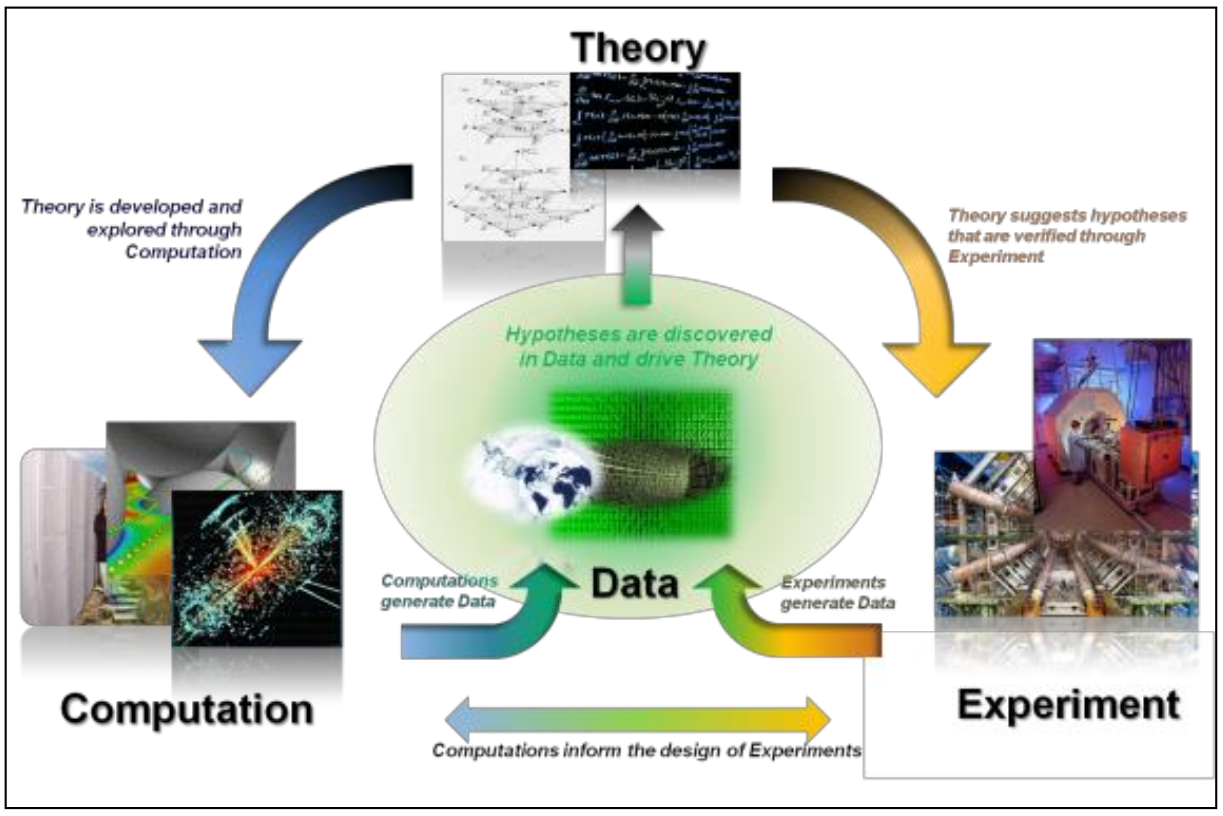
\includegraphics[height=2.30in,width=3.70in]{Figures/Four_Model_1.png}
%%\caption{\tiny \textrm{Pseudopotential for metallic sodium, based on the empty core model and screened by the Thomas-Fermi dielectric function.}}%(与文献\cite{EPJB33-47_2003}图1对比)
%\label{Four_Model_1}
%\end{figure}
%科学的新驱动力:~\textcolor{red}{密集数据}+\textcolor{red}{人工智能}\\
%}
%
%-----------------------------------------------------------------------------------------------------------------------------------------------------------------------%
